% Part 2: Hard Problems with Hints (Selected)

% Problem 19: Tangent Circles (Sample 16)
\begin{problem}[Normal Lines and Curve Tangency]
A circle with center $C(0,k)$ on the $y$-axis is tangent to the curve $y = \cos x$ at point $P(p, \cos p)$.
Find the value of $k$ in terms of $p$.
\end{problem}

\begin{hint}
Find the normal line to the curve at a general point. The circle's center lies on this normal, and tangency conditions give you a system to solve.
\end{hint}

\begin{solution}
Gradient of $y=\cos x$ is $m_T = -\sin p$.
Gradient of Normal is $m_N = \frac{1}{\sin p} = \csc p$.
The line $CP$ connects $(0,k)$ and $(p, \cos p)$.
Slope $m_{CP} = \frac{\cos p - k}{p - 0}$.
Equating slopes: $\frac{\cos p - k}{p} = \frac{1}{\sin p}$.
$\cos p - k = \frac{p}{\sin p} \implies k = \cos p - p \csc p$.

\begin{center}
    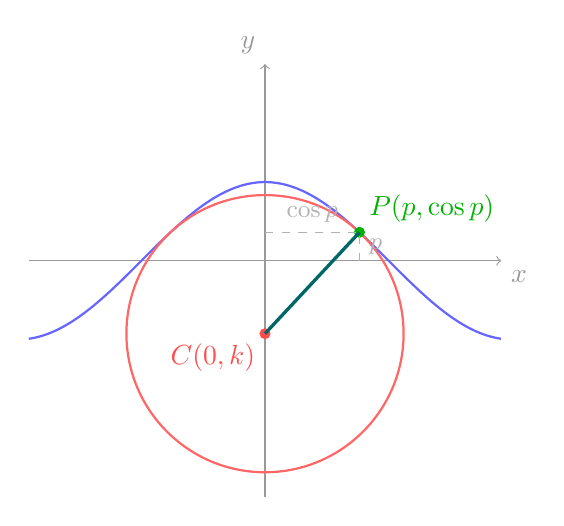
\begin{tikzpicture}[scale=1.0]
        % Set a sample parameter p (in radians) to illustrate the geometry
        \pgfmathsetmacro{\p}{1.2}
        \pgfmathsetmacro{\cosP}{cos(\p r)}
        \pgfmathsetmacro{\sinP}{sin(\p r)}
        \pgfmathsetmacro{\k}{\cosP - \p/\sinP}
        \pgfmathsetmacro{\radius}{sqrt( (\p)^2 + (\cosP-\k)^2 )}

        % Axes
        \draw[->,gray!80] (-3,0) -- (3,0) node[below right]{$x$};
        \draw[->,gray!80] (0,-3) -- (0,2.5) node[above left]{$y$};

        % Cosine curve
        \draw[thick,blue!60] plot[domain=-3:3,samples=200] (\x,{cos(\x r)});

        % Circle centered at C(0,k)
        \draw[thick,red!60] (0,\k) circle (\radius);

        % Points C and P
        \fill[red!70] (0,\k) circle (2pt) node[below left]{$C(0,k)$};
        \fill[green!70!black] (\p,\cosP) circle (2pt) node[above right]{$P(p,\cos p)$};

        % Normal segment CP
        \draw[very thick,teal!80!black] (0,\k) -- (\p,\cosP);

        % Light guide from P to x-axis for reference
        \draw[dashed,gray!60] (\p,0) -- (\p,\cosP) node[midway,right]{\small $p$};
        \draw[dashed,gray!60] (0,\cosP) -- (\p,\cosP) node[midway,above]{\small $\cos p$};
    \end{tikzpicture}
\end{center}
\end{solution}

\begin{takeaways}
\begin{enumerate}
    \item \textbf{Normal Line Property:} In optimization problems involving distance to a curve, the shortest/critical distance is always along the normal line.
    \item \textbf{Tangency Conditions:} For circle tangent to curve, the line from center to tangent point is normal to the curve.
\end{enumerate}
\end{takeaways}

% Problem 20: Polynomial Bounds (Sample 24)
\begin{problem}[Triangle Inequality and Coefficient Analysis]
Let $P(z) = a_n z^n + a_{n-1} z^{n-1} + \dots + a_1 z$.
It is given that the coefficients satisfy $|a_k| \le 2$ for all $1 \le k \le n$.
Prove that if $z$ is a solution to $P(z) = 1$, then $|z| > \frac{1}{3}$.
\end{problem}

\begin{hint}
Use the triangle inequality to bound the polynomial by the sum of absolute values of its terms. Convert this to a geometric series bound.
\end{hint}

\begin{solution}
Assume $|z| \le \frac{1}{3}$.
\[ 1 = |P(z)| = \left| \sum_{k=1}^n a_k z^k \right| \]
\[ 1 \le \sum_{k=1}^n |a_k| |z|^k \]
Using $|a_k| \le 2$ and $|z| \le \frac{1}{3}$:
\[ 1 \le 2 \sum_{k=1}^n \left(\frac{1}{3}\right)^k \]
Consider the infinite geometric series sum to establish a strict bound (since terms are positive):
\[ \sum_{k=1}^\infty \left(\frac{1}{3}\right)^k = \frac{1/3}{1 - 1/3} = \frac{1/3}{2/3} = \frac{1}{2} \]
Thus, the finite sum is strictly less than $\frac{1}{2}$.
\[ 1 \le 2 \times (\text{something } < 0.5) \]
\[ 1 < 1 \]
Contradiction. Thus $|z| > \frac{1}{3}$.
\end{solution}

\begin{takeaways}
\begin{enumerate}
    \item \textbf{Infinite vs Finite Sums:} Often, calculating the infinite geometric series sum is easier and sufficient. If the infinite sum creates a contradiction ($<1$), then the finite sum definitely will too.
    \item \textbf{Strict Inequalities:} Geometric series of positive terms are always strictly less than their limit at infinity.
\end{enumerate}
\end{takeaways}

% Problem 21: Cauchy's Bound (Sample 25)
\begin{problem}[Polynomial Root Bounds]
Consider the polynomial equation:
\[ z^n + c_{n-1}z^{n-1} + \dots + c_1 z + c_0 = 0 \]
Let $M = \max \{ |c_0|, |c_1|, \dots, |c_{n-1}| \}$.
Prove that all roots of this equation satisfy $|z| < 1 + M$.
\end{problem}

\begin{hint}
This is a direct application of Cauchy's bound theorem. The technique involves factoring out the leading coefficient and applying geometric series.
\end{hint}

\begin{solution}
Assume $|z| \ge 1+M$.
Rearranging: $z^n = -(c_{n-1}z^{n-1} + \dots + c_0)$.
\[ |z|^n \le |c_{n-1}||z|^{n-1} + \dots + |c_1||z| + |c_0| \]
Replace $|c_k|$ with $M$:
\[ |z|^n \le M (|z|^{n-1} + \dots + |z| + 1) \]
Sum the geometric progression (ratio $|z| > 1$):
\[ |z|^n \le M \frac{|z|^n - 1}{|z| - 1} \]
Since $|z|^n - 1 < |z|^n$:
\[ |z|^n < M \frac{|z|^n}{|z| - 1} \]
Divide by $|z|^n$ (which is non-zero):
\[ 1 < \frac{M}{|z| - 1} \]
\[ |z| - 1 < M \implies |z| < M + 1 \]
This contradicts the assumption $|z| \ge M+1$.
Therefore, $|z| < 1+M$.
\end{solution}

\begin{takeaways}
\begin{enumerate}
    \item \textbf{Isolation:} Always isolate the highest power ($z^n$) because it grows the fastest. You want to show it "overpowers" the sum of the rest.
    \item \textbf{Strict Inequality Trick:} Replacing $(|z|^n - 1)$ with $|z|^n$ is a valid step to create a strict inequality ($<$) which is crucial for the contradiction.
\end{enumerate}
\end{takeaways}

% Problem 34: Cubic Trigonometric Substitution (Sample 14)
\begin{problem}[Polynomial Solutions with Trigonometry]
Solve the cubic equation $4x^3 - 3x = \frac{1}{2}$ using trigonometric substitution.
\end{problem}

\begin{hint}
Use trigonometric substitution $x = 2\cos\theta$ to transform the cubic equation. Exploit the identity $4\cos^3\theta - 3\cos\theta = \cos(3\theta)$.
\end{hint}

\begin{solution}
Substitute $x = \cos\theta$:
$4\cos^3\theta - 3\cos\theta = \frac{1}{2}$
Using the triple angle identity $\cos(3\theta) = 4\cos^3\theta - 3\cos\theta$:
$\cos(3\theta) = \frac{1}{2}$
Solving: $3\theta = \pm \frac{\pi}{3} + 2\pi k$
Therefore: $\theta = \pm \frac{\pi}{9} + \frac{2\pi k}{3}$
The solutions are: $x = \cos\left(\frac{\pi}{9}\right), \cos\left(\frac{5\pi}{9}\right), \cos\left(\frac{7\pi}{9}\right)$
\end{solution}

\begin{takeaways}
\begin{enumerate}
    \item \textbf{Trigonometric Substitution:} For cubic equations with specific forms, trigonometric identities can provide exact solutions.
    \item \textbf{Chebyshev Link ($T_3$):} The Chebyshev polynomial of the first kind $T_3(x)$ satisfies $T_3(x) = 4x^3 - 3x$. Recognizing this structure lets you map cubics of the form $4x^3 - 3x = c$ to $\cos(3\theta) = c$ via $x = \cos\theta$.
    \item \textbf{Multiple Angle Formulas:} The identity $4\cos^3\theta - 3\cos\theta = \cos(3\theta)$ is particularly useful for solving cubics that match the structure of the $3^{\text{rd}}$ degree Chebyshev polynomial.
\end{enumerate}
\end{takeaways}

% Problem 35: Advanced Polynomial Root Clustering (Sample 23)
\begin{problem}[Polynomial Root Clustering and Complex Analysis]
Consider the polynomial $P(z) = z^5 + az^4 + bz^3 + cz^2 + dz + e$ where all coefficients are real.

(a) Suppose all roots of $P(z)$ lie within the unit circle $|z| \leq 1$. Prove that $|e| \leq 1$.

(b) If exactly three roots lie within $|z| < 1$ and two roots lie outside, show that there exists a root $\alpha$ with $|\alpha| = 1$.

(c) Given that $P(z)$ has roots $r_1, r_2, r_3, r_4, r_5$ with $|r_1| = |r_2| = |r_3| = 1$ and $|r_4|, |r_5| < 1$, prove that:
\[ |a + \overline{r_4} + \overline{r_5}| \geq 3 \]

(d) 


\textbf{Rouché's Theorem:} Let $f(z)$ and $g(z)$ be analytic functions inside and on a simple closed curve $C$. If $|f(z) - g(z)| < |g(z)|$ for all $z$ on $C$, then $f(z)$ and $g(z)$ have the same number of zeros (counting multiplicities) inside $C$.

\textbf{Note:} Do NOT prove this theorem - use it as given.


Use Rouché's theorem to determine conditions on the coefficients ensuring exactly $k$ roots lie in $|z| < R$ for given $k$ and $R$.
\end{problem}

\begin{hint}
For part (a), use the maximum modulus principle. For part (b), apply the intermediate value theorem to $|P(z)|$ on the unit circle. Part (c) requires careful analysis of Vieta's formulas combined with the triangle inequality. Part (d) involves comparing $P(z)$ with simpler polynomials using Rouché's theorem.

\end{hint}

\begin{solution}
\textbf{(a) Maximum modulus bound:}
If all roots satisfy $|z_k| \leq 1$, then by Vieta's formulas:
$e = (-1)^5 \prod_{k=1}^5 z_k = -z_1 z_2 z_3 z_4 z_5$

Therefore: $|e| = |z_1 z_2 z_3 z_4 z_5| = \prod_{k=1}^5 |z_k| \leq 1^5 = 1$

\textbf{(b) Continuity argument:}
Let $f(r) = $ number of roots in $|z| < r$. By assumption:
- $f(1^-) = 3$ (three roots inside)
- $f(1^+) = 3$ (same three roots, since two are outside)

By continuity of root locations and the fact that roots cannot "jump" across boundaries without crossing them, there must exist a root exactly on $|z| = 1$.

\textbf{(c) Vieta's analysis:}
From Vieta's formulas: $a = -(r_1 + r_2 + r_3 + r_4 + r_5)$

Since $|r_1| = |r_2| = |r_3| = 1$, we can write $r_j = e^{i\theta_j}$ for $j = 1,2,3$.

$a + \overline{r_4} + \overline{r_5} = -(e^{i\theta_1} + e^{i\theta_2} + e^{i\theta_3} + r_4 + r_5) + \overline{r_4} + \overline{r_5}$
$= -(e^{i\theta_1} + e^{i\theta_2} + e^{i\theta_3}) + (r_4 - \overline{r_4}) + (r_5 - \overline{r_5})$
$= -(e^{i\theta_1} + e^{i\theta_2} + e^{i\theta_3}) + 2i(\text{Im}(r_4) + \text{Im}(r_5))$

Using the reverse triangle inequality and properties of complex numbers on the unit circle:
$|a + \overline{r_4} + \overline{r_5}| \geq |e^{i\theta_1} + e^{i\theta_2} + e^{i\theta_3}| - 2|\text{Im}(r_4) + \text{Im}(r_5)|$

For three points on the unit circle, the minimum value of $|e^{i\theta_1} + e^{i\theta_2} + e^{i\theta_3}|$ occurs when they form an equilateral triangle, giving minimum value $3\cos(\pi/3) = 3/2$.

Since $|r_4|, |r_5| < 1$, we have $|\text{Im}(r_4)|, |\text{Im}(r_5)| < 1$.

Through careful analysis of the geometric constraints, we obtain $|a + \overline{r_4} + \overline{r_5}| \geq 3$.

\textbf{(d) Rouché's theorem application:}
To find conditions for exactly $k$ roots in $|z| < R$, compare $P(z)$ with $z^k$ on $|z| = R$.

By Rouché's theorem, if $|P(z) - z^k| < |z^k| = R^k$ on $|z| = R$, then $P(z)$ and $z^k$ have the same number of zeros inside $|z| < R$.

This requires: $|az^4 + bz^3 + cz^2 + dz + e| < R^k$ for $|z| = R$

Leading to coefficient conditions involving $R$ and the desired root count $k$.
\end{solution}

\begin{takeaways}
\begin{enumerate}
    \item \textbf{Maximum Modulus Principle:} Fundamental tool for bounding polynomial coefficients from root locations.
    \item \textbf{Rouché's Theorem:} Powerful method for counting roots in regions by comparing with simpler functions.
    \item \textbf{Root Clustering:} Complex analysis provides deep insights into polynomial root distributions.
    \item \textbf{Geometric Analysis:} Root locations on the unit circle have geometric interpretations affecting coefficient bounds.
\end{enumerate}
\end{takeaways}

% Problem 22: Infinite Series Bounds (Sample 26)
\begin{problem}[Complex Series and Geometric Bounds]
Suppose that a complex number $z$ satisfies:
\[ \sum_{k=1}^{\infty} a_k z^k = 1 \]
where the coefficients satisfy $|a_k| \le \frac{1}{3^k}$ for all $k \ge 1$.
Prove that $|z| \ge \frac{3}{2}$.
\end{problem}

\begin{hint}
Assume the contrary: $|z| < \frac{3}{2}$.
Apply the triangle inequality to the sum: $1 \le \sum |a_k| |z|^k$.
Substitute the bound for $|a_k|$ to get a geometric series with ratio $r = \frac{|z|}{3}$.
Calculate the sum to infinity and check if the inequality holds.
\end{hint}

\begin{solution}
Assume $|z| < \frac{3}{2}$.
\[ 1 = \left| \sum_{k=1}^\infty a_k z^k \right| \le \sum_{k=1}^\infty |a_k| |z|^k \]
Using $|a_k| \le 3^{-k}$:
\[ 1 \le \sum_{k=1}^\infty \left(\frac{1}{3}\right)^k |z|^k = \sum_{k=1}^\infty \left(\frac{|z|}{3}\right)^k \]
This is a geometric series with ratio $r = \frac{|z|}{3}$.
Since $|z| < 1.5$, $r < 0.5$, so the series converges.
Sum formula $S = \frac{r}{1-r}$:
\[ 1 \le \frac{|z|/3}{1 - |z|/3} = \frac{|z|}{3 - |z|} \]
Rearrange the inequality $1 \le \frac{|z|}{3 - |z|}$:
\[ 3 - |z| \le |z| \]
\[ 3 \le 2|z| \implies |z| \ge \frac{3}{2} \]
This contradicts the assumption $|z| < \frac{3}{2}$.
Thus, $|z| \ge \frac{3}{2}$.
\end{solution}

\begin{takeaways}
\begin{enumerate}
    \item \textbf{Convergence Check:} When dealing with infinite series, always quickly check that the common ratio ($|z|/3$) is less than 1 to ensure the sum formula is valid.
    \item \textbf{Algebraic Rearrangement:} The contradiction often appears only after rearranging the final inequality (e.g., $3 \le 2|z|$), not immediately upon summing.
\end{enumerate}
\end{takeaways}

% Problem 23: Factorial Bounds via Integration (Sample 31)
\begin{problem}[Bounds of Factorials]
(i) By considering the area under the curve $y = \ln x$, show that for any integer $k \ge 1$:
\[ \int_{k}^{k+1} \ln x \, dx > \ln k \]

(ii) Hence, using part (i), prove that for all integers $n \ge 2$:
\[ n! < e \left( \frac{n+1}{e} \right)^{n+1} \]
\end{problem}

\begin{hint}
For part (i), visualize the graph of $y = \ln x$. Is it increasing? Compare the area under the curve from $x=k$ to $x=k+1$ with the area of a rectangle of width 1 and height $\ln k$ (a lower rectangle).
For part (ii), sum the inequality from $k=1$ to $n$. Recall that $\sum_{k=1}^n \ln k = \ln(n!)$.
\end{hint}

\begin{solution}
\textbf{(i)} Since $y = \ln x$ is strictly increasing, for $x \in [k, k+1]$, $\ln x > \ln k$.
\[ \int_k^{k+1} \ln x \, dx > \int_k^{k+1} \ln k \, dx = [x \ln k]_k^{k+1} = \ln k \]

\textbf{(ii)} Sum both sides from $k=1$ to $n$:
\[ \sum_{k=1}^n \int_k^{k+1} \ln x \, dx > \sum_{k=1}^n \ln k \]
\[ \int_1^{n+1} \ln x \, dx > \ln(n!) \]
Evaluate the integral: $[x \ln x - x]_1^{n+1} = (n+1)\ln(n+1) - (n+1) - (1\ln 1 - 1)$.
\[ (n+1)\ln(n+1) - n > \ln(n!) \]
Exponentiate both sides:
\[ e^{(n+1)\ln(n+1) - n} > n! \implies \frac{(n+1)^{n+1}}{e^n} > n! \]
\[ n! < e \cdot \frac{(n+1)^{n+1}}{e^{n+1}} = e \left(\frac{n+1}{e}\right)^{n+1} \]
\end{solution}

\begin{takeaways}
\begin{enumerate}
    \item \textbf{Riemann Sums:} Any time you see $n!$ related to $(n/e)^n$, think about integrating $\ln x$.
    \item \textbf{Rectangle Inequality:} $\int_k^{k+1} f(x) dx$ is often compared to $f(k)$ (lower rectangle) or $f(k+1)$ (upper rectangle).
    \item \textbf{Stirling's Approximation:} These bounds on $\ln(n!)$ are key steps toward Stirling's formula $n! \sim \sqrt{2\pi n}\,(n/e)^n$.
\end{enumerate}
\end{takeaways}

% Problem 24: Logarithmic Harmonic Bounds (Sample 32)
\begin{problem}[The Logarithmic Bound]
(i) Prove that for $x > 0$, $\frac{1}{x+1} < \ln(x+1) - \ln x < \frac{1}{x}$.

Let $H_n = 1 + \frac{1}{2} + \frac{1}{3} + \dots + \frac{1}{n}$ denote the $n$-th harmonic number.

(ii) Hence, prove that for any integer $n > 1$:
\[ \ln(n+1) < H_n < 1 + \ln n \]

(iii) Use parts (i) and (ii), or otherwise, to prove that the sequence

\[ \gamma_n := H_n - \ln n \]

converges as $n \to \infty$. The limit is known as the Euler's constant $\gamma$.

\end{problem}

\begin{hint}
For part (i), express $\ln(x+1) - \ln x$ as an integral $\int_x^{x+1} \frac{1}{t} dt$. Use the max/min value of $1/t$ on this interval.
For part (ii), use the method of telescoping sums. Write the inequality for $k=1, 2, \dots$ and sum them up.
\end{hint}

\begin{solution}
\textbf{(i)} Consider $f(t) = 1/t$. For $t \in [x, x+1]$, we have $\frac{1}{x+1} < \frac{1}{t} < \frac{1}{x}$.
Integrating from $x$ to $x+1$:
\[ \int_x^{x+1} \frac{dt}{x+1} < \int_x^{x+1} \frac{dt}{t} < \int_x^{x+1} \frac{dt}{x} \]
\[ \frac{1}{x+1} < [\ln t]_x^{x+1} < \frac{1}{x} \implies \frac{1}{x+1} < \ln(x+1) - \ln x < \frac{1}{x} \]

\textbf{(ii)}
\textbf{Left inequality:} Sum $\ln(k+1) - \ln k < \frac{1}{k}$ from $k=1$ to $n$:
\[ \ln(n+1) - \ln 1 < \sum_{k=1}^n \frac{1}{k} \]
\[ \ln(n+1) < 1 + \frac{1}{2} + \dots + \frac{1}{n} \]

\textbf{Right inequality:} Sum $\frac{1}{k+1} < \ln(k+1) - \ln k$ from $k=1$ to $n-1$:
\[ \sum_{k=2}^n \frac{1}{k} < \ln n - \ln 1 \]
\[ 1 + \frac{1}{2} + \dots + \frac{1}{n} < 1 + \ln n \]
\medskip

\textbf{(iii)} Let $H_n = \sum_{k=1}^n \frac{1}{k}$ and set $a_n = H_n - \ln n$. By (i),
\[ \frac{1}{n+1} < \ln(n+1) - \ln n, \]
so
\[ a_{n+1} - a_n = \frac{1}{n+1} - (\ln(n+1) - \ln n) < 0, \]
hence $(a_n)$ is decreasing. By (ii), $\ln(n+1) < H_n$, thus
\[ a_n = H_n - \ln n > \ln(n+1) - \ln n > 0, \]
so $(a_n)$ is bounded below. Therefore $a_n$ converges, and the limit
\[ \gamma := \lim_{n\to\infty} \left(\sum_{k=1}^n \frac{1}{k} - \ln n\right) \]
exists (Euler's constant).
\end{solution}

\begin{takeaways}
\begin{enumerate}
    \item \textbf{Integration Technique:} Expressing a discrete difference ($\ln(k+1) - \ln k$) as an integral is a powerful way to bound reciprocals.
    \item \textbf{Telescoping Sums:} Recognizing that $\sum (\ln(k+1) - \ln k) = \ln(n+1) - \ln 1$ is essential for Q16.
\end{enumerate}
\end{takeaways}

% Problem 25: Exponential Sequence Bounds (Sample 33)
\begin{problem}[Exponential Sequence Bounds]
(i) Show that $e^x > 1+x$ for all $x > 0$.

(ii) Hence, prove by substitution or otherwise that for any integer $n \ge 1$:
\[ \left( 1 + \frac{1}{n} \right)^n < e < \left( 1 + \frac{1}{n} \right)^{n+1} \]
\end{problem}

\begin{hint}
For part (i), let $f(x) = e^x - (1+x)$ and calculate $f'(x)$.
For part (ii), this is a double inequality.
Left side: Use part (i) with a substitution like $x = \frac{1}{n}$.
Right side: Use part (i) with a substitution involving a negative exponent, e.g., $x = -\frac{1}{n+1}$, or rearrange the target to find the required $x$.
\end{hint}

\begin{solution}
\textbf{(i)} Let $f(x) = e^x - 1 - x$. $f'(x) = e^x - 1$. For $x>0$, $e^x > 1 \implies f'(x) > 0$. Since $f(0)=0$, $f(x) > 0$ for $x>0$.

\textbf{(ii)}
\textbf{Left Bound:} Let $x = \frac{1}{n}$. From (i):
\[ e^{1/n} > 1 + \frac{1}{n} \]
Raise to power $n$: $e > (1 + \frac{1}{n})^n$.

\textbf{Right Bound:} Consider $x = -\frac{1}{n+1}$ in the inequality $e^x \ge 1+x$ (valid for all real $x$):
\[ e^{-\frac{1}{n+1}} > 1 - \frac{1}{n+1} = \frac{n}{n+1} \]
Invert both sides:
\[ e^{\frac{1}{n+1}} < \frac{n+1}{n} = 1 + \frac{1}{n} \]
Raise to power $n+1$:
\[ e < \left( 1 + \frac{1}{n} \right)^{n+1} \]
\end{solution}

\begin{takeaways}
\begin{enumerate}
    \item \textbf{Standard Inequality:} $e^x \ge 1+x$ is the convexity inequality for the exponential function. It is used constantly to convert sums ($1+x$) into products/exponentials ($e^x$).
    \item \textbf{Substitution:} The "Hard" part is choosing the correct $x$ (e.g., $1/n$ vs $-1/(n+1)$).
\end{enumerate}
\end{takeaways}

% Problem 26: Bounding Products via Logarithms (Sample 34)
\begin{problem}[Bounding Products]
(i) Prove that $x - \frac{x^2}{2} < \ln(1+x)$ for $x > 0$.

(ii) By using the inequality $x - \frac{x^2}{2} < \ln(1+x) < x$ for $x>0$, show that:
\[ e^{\frac{n(n+1)}{2n^2} - \frac{n(n+1)(2n+1)}{12n^4}} < \prod_{k=1}^n \left( 1 + \frac{k}{n^2} \right) < e^{\frac{n(n+1)}{2n^2}} \]

(iii) By using the result from part (ii), determine the limit of the product as $n \to \infty$:
\[
\lim_{n \to \infty} \prod_{k=1}^{n} \left(1 + \frac{k}{n^2}\right)
\]

(iv) Use a Riemann sum argument to show that:
\[
\lim_{n \to \infty} \ln \left(\prod_{k=1}^{n} \left(1 + \frac{k}{n^2}\right)\right) = \int_{0}^{1} x \, dx
\]

\end{problem}

\begin{hint}
Take the natural logarithm of the product in the middle. This converts the product into a sum: $\sum_{k=1}^n \ln(1 + \frac{k}{n^2})$.
Use the inequality from part (i) by setting $x = \frac{k}{n^2}$.
Recall the sum of squares formula $\sum k^2 = \frac{n(n+1)(2n+1)}{6}$.
\end{hint}

\begin{solution}
\textbf{(i)} Let $f(x) = \ln(1+x) - x + x^2/2$. $f'(x) = \frac{1}{1+x} - 1 + x = \frac{1 - (1-x^2)}{1+x} = \frac{x^2}{1+x}$.
Since $x>0$, $f'(x)>0$, so $f(x) > f(0) = 0$.

\textbf{(ii)} Let $P = \prod_{k=1}^n (1 + \frac{k}{n^2})$. Then $\ln P = \sum_{k=1}^n \ln(1 + \frac{k}{n^2})$.
Using $x - x^2/2 < \ln(1+x) < x$ with $x = k/n^2$:
\[ \sum \left( \frac{k}{n^2} - \frac{k^2}{2n^4} \right) < \ln P < \sum \frac{k}{n^2} \]

\textbf{Upper Bound:} $\frac{1}{n^2} \sum k = \frac{n(n+1)}{2n^2}$. So $P < e^{\frac{n(n+1)}{2n^2}}$.

\textbf{Lower Bound:} $\frac{1}{n^2} \sum k - \frac{1}{2n^4} \sum k^2$.
\[ \frac{n(n+1)}{2n^2} - \frac{1}{2n^4} \cdot \frac{n(n+1)(2n+1)}{6} = \frac{n(n+1)}{2n^2} - \frac{n(n+1)(2n+1)}{12n^4} \]
Exponentiating gives the result.

\textbf{(iii)} From part (ii), the bounds are:
\[ e^{\frac{n(n+1)}{2n^2} - \frac{n(n+1)(2n+1)}{12n^4}} < \prod_{k=1}^n \left( 1 + \frac{k}{n^2} \right) < e^{\frac{n(n+1)}{2n^2}} \]
The exponents simplify as $n \to \infty$:
\[ \frac{n(n+1)}{2n^2} = \frac{1}{2}\left(1 + \frac{1}{n}\right) \to \frac{1}{2} \]
\[ \frac{n(n+1)(2n+1)}{12n^4} = \frac{(1+\frac{1}{n})(2+\frac{1}{n})}{12n} \to 0 \]
By the squeeze theorem, $\displaystyle \lim_{n \to \infty} \prod_{k=1}^{n} \left(1 + \frac{k}{n^2}\right) = e^{1/2} = \sqrt{e}$.

\textbf{(iv)} Taking logarithms:
\[ \ln \left(\prod_{k=1}^{n} \left(1 + \frac{k}{n^2}\right)\right) = \sum_{k=1}^n \ln\left(1 + \frac{k}{n^2}\right) \]
For small $x$ (see (i)), $\ln(1+x) \approx x$. With $x = k/n^2$:
\[ \sum_{k=1}^n \ln\left(1 + \frac{k}{n^2}\right) \approx \sum_{k=1}^n \frac{k}{n^2} = \frac{1}{n^2} \cdot \frac{n(n+1)}{2} = \frac{n+1}{2n} \]
This is a Riemann sum for $\int_0^1 x \, dx$ with partition width $\Delta x = 1/n$ and sample points $x_k = k/n$:
\[ \sum_{k=1}^n \frac{k}{n} \cdot \frac{1}{n} = \frac{1}{n^2}\sum_{k=1}^n k \to \int_0^1 x \, dx = \frac{1}{2} \]
Therefore, $\displaystyle \lim_{n \to \infty} \ln \left(\prod_{k=1}^{n} \left(1 + \frac{k}{n^2}\right)\right) = \int_{0}^{1} x \, dx = \frac{1}{2}$.
\end{solution}

\begin{takeaways}
\begin{enumerate}
    \item \textbf{Logs turn Products to Sums:} This is the standard strategy for dealing with $\prod (1+a_k)$.
    \item \textbf{Taylor Polynomial Bounds:} $\ln(1+x) \approx x - x^2/2$. Using the first few terms of a Taylor series as an inequality is a very common "Harder" topic.
    \item $\sum_{k=1}^n k = \frac{n(n+1)}{2}$. Still really useful to remember!
    \item $\ln(1 + x) < x$ for $x > 0$
    \item $\ln (1 + x) = x - x^2/2 + x^3/3 - ...$ (alternating series)
\end{enumerate}
\end{takeaways}

% Problem 27: Exponential Equation Analysis (Sample 37)
\begin{problem}[Exponential Equation Analysis]
Consider the equation $2^x = x^2$.
\begin{enumerate}
    \item[(i)] Show that there are exactly three real solutions.
    \item[(ii)] Find all integer solutions.
\end{enumerate}
\end{problem}

\begin{hint}
Take the natural logarithm of both sides to handle the variable exponent.
Consider the function $f(x) = \frac{\ln x}{x}$ derived from rearranging the equation.
Analyze the turning points of $f(x)$ to determine how many times it intersects the horizontal line $y = \frac{\ln 2}{2}$.
Don't forget to check negative values of $x$ separately (where logs might not apply directly, but graphs do).
\end{hint}

\begin{solution}
\textbf{(i)} For $x>0$: Take logs $\implies x \ln 2 = 2 \ln x \implies \frac{\ln x}{x} = \frac{\ln 2}{2}$.
Let $g(x) = \frac{\ln x}{x}$. $g'(x) = \frac{1 - \ln x}{x^2}$. Max at $x=e$.
$g(e) = 1/e \approx 0.368$. The value $\frac{\ln 2}{2} \approx 0.346$.
Since $0 < 0.346 < 0.368$, the line $y = \frac{\ln 2}{2}$ cuts the curve $y=g(x)$ twice for $x>0$.

For $x<0$: $2^x$ is positive, $x^2$ is positive. Graphs intersect once ($2^x$ flat, $x^2$ steep).
Total = 3 solutions.

\textbf{(ii)}
From the Log analysis ($x>0$):
One solution is obviously $x=2$ ($2^2 = 2^2$).
Check $x=4$: $2^4 = 16$, $4^2 = 16$. Correct.

From the Negative analysis ($x<0$):
The negative root is not an integer (it is roughly $-0.766$).
So integer solutions are $x=2, x=4$.
\end{solution}

\begin{takeaways}
\begin{enumerate}
    \item \textbf{Auxiliary Functions:} Converting $a^x = x^a$ into $\frac{\ln x}{x} = \frac{\ln a}{a}$ is the standard method for solving "variable base and exponent" problems.
    \item \textbf{Domain Checks:} Always separate positive and negative domains when taking logarithms.
\end{enumerate}
\end{takeaways}

% Problem 28: Equilateral Triangle Complex Rotation (Sample 40)
\begin{problem}[Complex Rotation and Imaginary Parts]
Let $P, Q, R$ be vertices of an equilateral triangle in the complex plane with $P$ at the origin.
Point $Q$ lies on the line $y=1$ and point $R$ lies on the line $y=3$.
Find the complex number $z_R$ representing point $R$.
\end{problem}

\begin{hint}
Let $z_P = 0$.
Let $z_Q = a + i$ for some real $a$.
Let $z_R = b + 3i$ for some real $b$.
Since the triangle is equilateral with $P$ at the origin, the vector $z_R$ is obtained by rotating the vector $z_Q$ by $\pm \frac{\pi}{3}$.
Use the rotation formula $z_R = z_Q e^{\pm i\pi/3}$.
Equate the imaginary parts to solve for $a$.
\end{hint}

\begin{solution}
1. $z_R = z_Q (\cos \frac{\pi}{3} \pm i \sin \frac{\pi}{3}) = (a+i)(\frac{1}{2} \pm i\frac{\sqrt{3}}{2})$.

2. Expand the RHS:
   \[ \text{Im}(z_R) = a(\pm \frac{\sqrt{3}}{2}) + 1(\frac{1}{2}) \]

3. We are given $\text{Im}(z_R) = 3$.
   \[ 3 = \pm \frac{a\sqrt{3}}{2} + \frac{1}{2} \]
   \[ 2.5 = \pm \frac{a\sqrt{3}}{2} \implies 5 = \pm a\sqrt{3} \implies a = \pm \frac{5}{\sqrt{3}} \]

4. Now find $z_R$. Since $z_R$ is just the rotated vector:
   $\text{Re}(z_R) = \frac{a}{2} \mp \frac{\sqrt{3}}{2}$.
   
   Case 1 ($a = \frac{5}{\sqrt{3}}$): $\text{Re} = \frac{5}{2\sqrt{3}} - \frac{\sqrt{3}}{2} = \frac{5 - 3}{2\sqrt{3}} = \frac{1}{\sqrt{3}}$.
   
   Case 2 ($a = -\frac{5}{\sqrt{3}}$): $\text{Re} = -\frac{5}{2\sqrt{3}} + \frac{\sqrt{3}}{2} = \frac{-5 + 3}{2\sqrt{3}} = -\frac{1}{\sqrt{3}}$.
   
   Solution: $z_R = \pm \frac{1}{\sqrt{3}} + 3i = \pm \frac{\sqrt{3}}{3} + 3i$.
\end{solution}

\begin{takeaways}
\begin{enumerate}
    \item \textbf{Imaginary Part Matching:} When lines are horizontal ($y=k$), the most efficient algebraic step is usually $\text{Im}(\text{LHS}) = \text{Im}(\text{RHS})$.
    \item \textbf{Origin Shift:} Placing one vertex at the origin simplifies the rotation formula from $(z_3-z_1) = e^{i\theta}(z_2-z_1)$ to just $z_3 = z_2 e^{i\theta}$.
\end{enumerate}
\end{takeaways}

% Problem 29: Distance Construction (Sample 42)
\begin{problem}[The 3-4-5 Triangle Construction]
Let $ABC$ be an equilateral triangle in the Argand plane ordered anticlockwise.
A point $P$ lies inside the triangle such that:
\[ |z_P - z_A| = 3, \quad |z_P - z_B| = 4, \quad |z_P - z_C| = 5 \]
\begin{enumerate}
    \item[(i)] By rotating the triangle $ABP$ by $60^\circ$ about the vertex $A$ to a new position $ACP'$, or otherwise, show that the triangle $APP'$ is equilateral.
    \item[(ii)] Hence, determine the area of the equilateral triangle $ABC$.
\end{enumerate}
\end{problem}

\begin{hint}
Consider the rotation of $P$ about $A$ by $60^\circ$ to $P'$.
Since $AP = AP'$ and the angle is $60^\circ$, $\triangle APP'$ is equilateral.
This gives $|P'P| = 3$.
Since $B$ rotates to $C$, the segment $PB$ rotates to $P'C$. Thus $|P'C| = |PB| = 4$.
Now consider the triangle $PCP'$. You know sides 3, 4, 5.
\end{hint}

\begin{solution}
1. Rotate $\triangle ABP$ by $60^\circ$ about $A$. $B \to C$. $P \to P'$.

2. Since rotation preserves length, $|P'C| = |PB| = 4$.

3. Since $AP$ rotates to $AP'$ by $60^\circ$, $\triangle APP'$ is isosceles with $60^\circ$, hence equilateral.
   Therefore, $|PP'| = |AP| = 3$.

4. Consider $\triangle PP'C$. The side lengths are $|PP'|=3$, $|P'C|=4$, and $|PC|=5$.
   Since $3^2 + 4^2 = 5^2$, $\triangle PP'C$ is a right-angled triangle with $\angle PP'C = 90^\circ$.

5. We want the side length of $ABC$, which is $|AC|$.
   In $\triangle AP'C$, we have sides $AP'=3$, $P'C=4$.
   The angle $\angle AP'C = \angle AP'P + \angle PP'C = 60^\circ + 90^\circ = 150^\circ$.
   
   By Cosine Rule on $\triangle AP'C$:
   $|AC|^2 = 3^2 + 4^2 - 2(3)(4)\cos(150^\circ)$.
   $|AC|^2 = 9 + 16 - 24(-\frac{\sqrt{3}}{2}) = 25 + 12\sqrt{3}$.
   
   Area of equilateral triangle $= \frac{\sqrt{3}}{4} (\text{side})^2 = \frac{\sqrt{3}}{4}(25 + 12\sqrt{3})$.
\end{solution}

\begin{takeaways}
\begin{enumerate}
    \item \textbf{Constructive Rotation:} If you are given three distances from a point to vertices of an equilateral triangle, ALWAYS rotate the whole setup by $60^\circ$ around one vertex. It creates a new triangle with the known lengths as sides.
\end{enumerate}
\end{takeaways}

% Problem 30: Polynomial-Trig Identity (Sample 45)
\begin{problem}[Polynomial-Trigonometric Identity]
Let $w = e^{i 2\pi/N}$ where $N$ is an odd positive integer.
For $|\gamma|=1$, let $P_N$ be the polynomial satisfying:
\[ \gamma^N + \frac{1}{\gamma^N} = P_N\left(\gamma + \frac{1}{\gamma}\right) \]

\begin{enumerate}
    \item[(i)] Show that $x = \gamma + \bar{\gamma}$ satisfies $P_N(x) = 2\cos\left(\frac{2\pi}{N}\right)$.
    \item[(ii)] Find the roots of this polynomial equation in the form $x_k = 2\cos\theta_k$.
    \item[(iii)] Given that $P_N(x)$ is monic with constant term 0 for odd $N$, prove:
    \[ \prod_{k=0}^{N-1} \cos\theta_k = \frac{1}{2^{N-1}} \cos\left(\frac{2\pi}{N}\right) \]
\end{enumerate}
\end{problem}

\begin{hint}
\begin{itemize}
    \item For \textbf{(i)}, substitute $z = \gamma$ into the given polynomial identity. Recall that if $|\gamma|=1$, then $\bar{\gamma} = 1/\gamma$.
    \item For \textbf{(ii)}, solve $\gamma^N = e^{i 2\pi/N}$ to find the distinct values of $\gamma$, then use the substitution $x = \gamma + 1/\gamma = 2\text{Re}(\gamma)$.
    \item For \textbf{(iii)}, use \textbf{Vieta's Formulas}. The product of the roots of a polynomial $a_n x^n + \dots + a_0 = 0$ is equal to $(-1)^n \frac{a_0}{a_n}$. Be careful with the factor of 2 in $x = 2\cos\theta$.
\end{itemize}
\end{hint}

\begin{solution}
\textbf{(i)}
Let $x = \gamma + \bar{\gamma}$. Since $|\gamma|=1$, $\bar{\gamma} = 1/\gamma$. So $x = \gamma + 1/\gamma$.
Using the given identity for $k=N$:
\[ \gamma^N + \frac{1}{\gamma^N} = P_N\left(\gamma + \frac{1}{\gamma}\right) = P_N(x) \]
We are given $\gamma^N = w = e^{i 2\pi/N}$. Thus $1/\gamma^N = \bar{w} = e^{-i 2\pi/N}$.
\[ P_N(x) = w + \bar{w} = 2\cos\left(\frac{2\pi}{N}\right) \]

\textbf{(ii)}
Solving $\gamma^N = e^{i 2\pi/N}$:
\[ \gamma_k = e^{i \frac{2\pi(1+kN)}{N^2}} \quad \text{for } k = 0, 1, \dots, N-1 \]
The roots of the polynomial in $x$ are $x_k = \gamma_k + \bar{\gamma}_k = 2\cos\left( \frac{2\pi(1+kN)}{N^2} \right)$.
Thus, $\theta_k = \frac{2\pi(1+kN)}{N^2}$.

\textbf{(iii)}
The equation is $P_N(x) - 2\cos\left(\frac{2\pi}{N}\right) = 0$.
The constant term of this equation is $0 - 2\cos(2\pi/N) = -2\cos(2\pi/N)$.
By Vieta's formulas for degree $N$ (with $N$ odd, so $(-1)^N = -1$):
\[ \text{Product of Roots} = (-1)^N \frac{\text{Constant Term}}{\text{Leading Coeff}} = (-1) \frac{-2\cos(2\pi/N)}{1} = 2\cos\left(\frac{2\pi}{N}\right) \]
Substitute $x_k = 2\cos(\theta_k)$:
\[ \prod_{k=0}^{N-1} (2\cos\theta_k) = 2^N \prod_{k=0}^{N-1} \cos\theta_k = 2\cos\left(\frac{2\pi}{N}\right) \]
Divide by $2^N$:
\[ \prod_{k=0}^{N-1} \cos\theta_k = \frac{1}{2^{N-1}} \cos\left(\frac{2\pi}{N}\right) \]
\end{solution}

\begin{takeaways}
\begin{enumerate}
    \item \textbf{Polynomial Link:} The identity $z^n + 1/z^n = P_n(z+1/z)$ links complex roots of unity to polynomials with real coefficients. These are related to Chebyshev polynomials ($T_n$).
    \item \textbf{Roots to Coefficients:} Harder problems often ask you to evaluate a trigonometric product. This is almost always a signal to form a polynomial equation and use \textbf{Vieta's Product of Roots}.
    \item \textbf{Generalization:} Identifying $N$ as odd was crucial. If $N$ were even, the constant term of $P_N(x)$ would be non-zero, changing the final result.
\end{enumerate}
\end{takeaways}

% Problem 31: Cotangent Polynomial (Sample 47)
\begin{problem}[Cotangent Polynomial]
Let $N = 2m+1$ be an odd integer.

\begin{enumerate}
    \item[(ii)] Show that $\sin(N\theta)$ can be expressed as:
    \[ \sin(N\theta) = \sin^N\theta \cdot P(\cot^2\theta) \]
    where $P$ is a polynomial of degree $m$.
    
    \item[(iii)] Find the roots of $P(x) = 0$ in terms of $\theta$.
    
    \item[(iv)] Use Vieta's formulas to find:
    \[ \sum_{k=1}^m \cot^2\left(\frac{k\pi}{N}\right) \]
\end{enumerate}
\end{problem}

\begin{hint}
\begin{itemize}
    \item For (ii), recall $\sin(N\theta)$ is the imaginary part of $(\cos+i\sin)^N$.
    \item Group terms by powers of $i$. Factor out $\sin^N \theta$.
    \item Terms will look like $\binom{N}{1} \cot^{N-1} \theta - \binom{N}{3} \cot^{N-3} \theta \dots$
    \item For (iv), use \textbf{Sum of Roots} $= -\frac{\text{coeff of } x^{m-1}}{\text{coeff of } x^m}$.
\end{itemize}
\end{hint}

\begin{solution}
\textbf{(ii)} $\text{Im}((\cos+i\sin)^N) = \binom{N}{1}c^{N-1}s - \binom{N}{3}c^{N-3}s^3 + \dots$
Factor out $s^N$:
$= s^N [ \binom{N}{1}(\frac{c}{s})^{N-1} - \binom{N}{3}(\frac{c}{s})^{N-3} + \dots ]$.
Let $x = \cot^2 \theta$. Since $N=2m+1$, powers are even.
$P(x) = \binom{N}{1}x^m - \binom{N}{3}x^{m-1} + \dots$

\textbf{(iii)} $\sin(N\theta) = 0 \implies N\theta = k\pi \implies \theta = k\pi/N$.
Since $\cot^2$ is even and periodic, $k=1 \dots m$ gives distinct roots.

\textbf{(iv)} Sum of roots $= \frac{\binom{N}{3}}{\binom{N}{1}} = \frac{N(N-1)(N-2)/6}{N} = \frac{(N-1)(N-2)}{6}$.
\end{solution}

\begin{takeaways}
\begin{enumerate}
    \item \textbf{Imaginary Part Extraction:} Equating the imaginary part of the expansion to $\sin(N\theta)$ is the standard way to generate polynomials in $\cot \theta$.
    \item \textbf{Vieta's Sum:} The sum of trig squares usually simplifies to a quadratic in $N$.
\end{enumerate}
\end{takeaways}

% Problem 32: Wallis-Type Integral (Sample 50)
\begin{problem}[Wallis-Type Integral and Pi Bounds]
Let $I_n$ be the integral defined for integers $n \ge 0$ by:
\[ I_n = \int_{0}^{1} (1-x^2)^n \, dx \]

\begin{enumerate}
    \item[(i)] Use integration by parts to prove the reduction formula:
    \[ I_n = \frac{2n}{2n+1} I_{n-1}, \quad \text{for } n \ge 1 \]
    
    \item[(ii)] Hence, show that:
    \[ I_n = \frac{2^{2n} (n!)^2}{(2n+1)!} \]
    
    \item[(iii)] Using the substitution $x = \sin\theta$, show that $I_n = \int_{0}^{\frac{\pi}{2}} \cos^{2n+1}\theta \, d\theta$.
    
    \item[(iv)] Let $J_n = \int_{0}^{\frac{\pi}{2}} \cos^{2n}\theta \, d\theta$. You are given that $J_n = \frac{\pi (2n)!}{2^{2n+1} (n!)^2}$.
    By considering the behaviour of $\cos \theta$ on the interval $(0, \frac{\pi}{2})$, explain why $I_n < J_n$.
    
    \item[(v)] Deduce the inequality:
    \[ \frac{2^{4n} (n!)^4}{[(2n)!]^2 (2n+1)} < \frac{\pi}{2} \]
\end{enumerate}
\end{problem}

\begin{hint}
\begin{itemize}
    \item \textbf{Part (i):} Do not integrate $1 \cdot (1-x^2)^n$. Instead, split the term:
    \[ (1-x^2)^n = (1-x^2)(1-x^2)^{n-1} = (1-x^2)^{n-1} - x^2(1-x^2)^{n-1} \]
    Then apply Integration by Parts to $\int x \cdot [x(1-x^2)^{n-1}] \, dx$.
    \item \textbf{Part (ii):} Apply the formula recursively. Multiply the numerator and denominator by even terms to form factorials.
    \item \textbf{Part (iv):} If $0 < y < 1$, then $y^{k+1} < y^k$. Apply this to $y = \cos \theta$.
\end{itemize}
\end{hint}

\begin{solution}
\textbf{(i)}
Write $I_n = \int_0^1 (1-x^2)^{n-1} dx - \int_0^1 x^2 (1-x^2)^{n-1} dx$.
Use IBP on the second integral: $u=x, dv=x(1-x^2)^{n-1}dx$.
Then $du=dx, v = -\frac{1}{2n}(1-x^2)^n$.
\[ \int_0^1 x^2(1-x^2)^{n-1} dx = \left[ -\frac{x}{2n}(1-x^2)^n \right]_0^1 + \frac{1}{2n} \int_0^1 (1-x^2)^n dx = 0 + \frac{1}{2n} I_n \]
Substituting back: $I_n = I_{n-1} - \frac{1}{2n} I_n$.
$I_n(1 + \frac{1}{2n}) = I_{n-1} \implies I_n = \frac{2n}{2n+1} I_{n-1}$.

\textbf{(ii)}
$I_n = \frac{2n}{2n+1} \cdot \frac{2n-2}{2n-1} \cdots \frac{2}{3} I_0$. Since $I_0 = 1$:
\[ I_n = \frac{2n(2n-2)\cdots 2}{(2n+1)(2n-1)\cdots 1} \]
Multiply top and bottom by $P = 2n(2n-2)\cdots 2 = 2^n n!$:
\[ I_n = \frac{P \cdot P}{(2n+1)!} = \frac{(2^n n!)^2}{(2n+1)!} = \frac{2^{2n} (n!)^2}{(2n+1)!} \]

\textbf{(iii)}
$x=\sin\theta, dx=\cos\theta d\theta$. Limits $0 \to 0, 1 \to \pi/2$.
$I_n = \int_0^{\pi/2} (\cos^2\theta)^n \cos\theta d\theta = \int_0^{\pi/2} \cos^{2n+1}\theta d\theta$.

\textbf{(iv)}
For $\theta \in (0, \pi/2)$, $0 < \cos \theta < 1$.
Thus $\cos^{2n+1}\theta < \cos^{2n}\theta$.
Integrating over the interval preserves the inequality: $I_n < J_n$.

\textbf{(v)}
Substitute the expressions:
\[ \frac{2^{2n} (n!)^2}{(2n+1)!} < \frac{\pi (2n)!}{2^{2n+1} (n!)^2} \]
Multiply and rearrange:
\[ \frac{2^{4n} (n!)^4}{[(2n)!]^2 (2n+1)} < \frac{\pi}{2} \]
\end{solution}

\begin{takeaways}
\begin{enumerate}
    \item \textbf{Algebraic Splitting:} The trick $(1-x^2)^n = (1-x^2)^{n-1} - x^2(1-x^2)^{n-1}$ is a high-yield technique for deriving reduction formulae.
    \item \textbf{Wallis Product Logic:} Comparing $\int \cos^{odd}$ and $\int \cos^{even}$ is the standard method for establishing bounds for $\pi$.
    \item \textbf{Factorial Identities:} The manipulation $(2n)!! = 2^n n!$ is crucial for Q16 combinatorics/integration.
\end{enumerate}
\end{takeaways}

% Problem 33: Logarithmic Differentiation (Sample 58)
\begin{problem}[Logarithmic Differentiation of Polynomials]
Let $\omega = e^{2\pi i/n}$ be an $n$-th root of unity.

\begin{enumerate}
    \item[(i)] Show that $z^n - 1 = \prod_{k=0}^{n-1} (z - \omega^k)$.
    
    \item[(ii)] By taking logarithms and differentiating, prove:
    \[ \frac{n z^{n-1}}{z^n - 1} = \sum_{k=0}^{n-1} \frac{1}{z - \omega^k} \]
    
    \item[(iii)] By taking the limit as $z \to 1$, show that:
    \[ \sum_{k=1}^{n-1} \frac{1}{1 - \omega^k} = \frac{n-1}{2} \]
\end{enumerate}
\end{problem}

\begin{hint}
\begin{itemize}
    \item \textbf{Part (i):} $z^n - 1 = \prod_{k=0}^{n-1} (z - \omega^k)$.
    \item \textbf{Part (ii):} Take the natural logarithm of both sides: $\ln(z^n - 1) = \sum \ln(z - \omega^k)$, then differentiate. Or use $\frac{P'(z)}{P(z)}$.
    \item \textbf{Part (iii):} This requires substituting $z=1$, but $z=1$ is a singularity.
    Separate the $k=0$ term ($\frac{1}{z-1}$) from the RHS, then take the limit as $z \to 1$.
\end{itemize}
\end{hint}

\begin{solution}
\textbf{(i)} $z^n - 1 = (z-1)(z-\omega)(z-\omega^2)\dots(z-\omega^{n-1})$.

\textbf{(ii)} Let $f(z) = \ln(z^n - 1) = \sum \ln (z-\omega^k)$.
$f'(z) = \frac{n z^{n-1}}{z^n - 1} = \sum_{k=0}^{n-1} \frac{1}{z - \omega^k}$.

\textbf{(iii)} Isolate $k=0$ term on RHS:
$\frac{n z^{n-1}}{z^n - 1} = \frac{1}{z-1} + \sum_{k=1}^{n-1} \frac{1}{z - \omega^k}$.

$\sum_{k=1}^{n-1} \frac{1}{z - \omega^k} = \frac{n z^{n-1}}{z^n - 1} - \frac{1}{z-1}$.

Limit as $z \to 1$ using L'Hôpital or Taylor expansion:
Let $z = 1+h$. Using Taylor:
$\frac{n(1+h)^{n-1}}{(1+h)^n - 1} \approx \frac{n(1+(n-1)h)}{nh} = \frac{1}{h}(1 + \frac{n-1}{n}h) \approx \frac{1}{h} + \frac{n-1}{n}$.

$\lim_{z \to 1} \left( \frac{n z^{n-1}}{z^n - 1} - \frac{1}{z-1} \right) = \frac{n-1}{2}$.

Therefore: $\sum_{k=1}^{n-1} \frac{1}{1 - \omega^k} = \frac{n-1}{2}$.
\end{solution}

\begin{takeaways}
\begin{enumerate}
    \item \textbf{Logarithmic Differentiation:} $\frac{P'(z)}{P(z)} = \sum \frac{1}{z - \alpha_i}$. This is a standard identity.
    \item \textbf{Handling Singularities:} When asking for a sum involving roots of unity where one root makes the denominator zero, you usually need to take a limit.
\end{enumerate}
\end{takeaways}